\documentclass[a4paper,10pt]{article}
\usepackage[utf8]{inputenc}
\usepackage{hyperref}
\usepackage{graphicx}
\usepackage{amssymb}
\usepackage{amsmath}
\usepackage[margin=0.7in]{geometry}

%opening
\title{Combining Companies House and ONS data to build a detailed granular dataset of UK Companies}
\author{Alfred Holmes}
\date{September 2018}
\begin{document}


\maketitle
\begin{abstract}Companies House release the accounts (turnover, net assets) of 75\% of UK companies and basic data (location, age) of all UK companies. Assuming these companies are a representative sample, it is then possible to combine this with ONS reports of employment and local units, with few assumptions, to assign each individual company a selection of local units, each with a number of employees to match the ONS data the years 2012 - 2018. 
\end{abstract}
 
\section{Introduction}
Contemporary economic modeling requires detailed granular data. Typically highly granular data is not available due to difficulties collecting such data or privacy issues in releasing the information. In the case of UK companies data, an ideal dataset would contain the size (employment, turnover, net assets) along with location through time and branches of the companies operating in the UK. Companies House gives the net assets of most companies, and the turnovers of large companies. If we assume that the turnover for a business in a particular industry correlates strongly with employment, then using the employment size distributions from ONS it is possible to construct such a dataset.

\subsection{Companies House}
Companies house provides three sources of detailed data. Each month they release a \href{http://download.companieshouse.gov.uk/en_output.html}{snapshot} of active companies, containing the registered office location, age, SIC code and some other less relevant information. Unfortunately they do not release historic versions of this snapshot, only the one for the current month, but it is possible to get historic versions (approximately one per year) through \href{https://web.archive.org/web/*/http://download.companieshouse.gov.uk/en_output.html}{archive.org}. From the series of snapshots we can infer low resolution company migration data, as well as a list of company IDs through time. The list of company IDs is useful because another source of data from companies house is the \href{https://developer.companieshouse.gov.uk/api/docs/}{JSON API} which, given a company ID, can be queried to get the individual filing history of companies. The filing history can be used to get the exact dates for company migrations, as well as reading the company accounts to measure the size of each company. The third source of data is the \href{http://download.companieshouse.gov.uk/historicmonthlyaccountsdata.html}{company account filings} (from 2008 - present) that are available to download, which is easier than querying each individual company. The company account filings also contain filings for dormant companies, potentially offering more historic data that just the snapshots when combined with the API.

\subsection{ONS}
In relation to the size of firms, ONS release yearly data on the sizes of firms by SIC code and by location (local authority) - they release the number of enterprises and local units with sizes in particular intervals. They also release the employment totals for the public sector and private sector in each local authority, as well as location look up tables to give the location (latitude and longitude) and the local authority of each postcode.


\subsection{Description of Terms}
Since there are different types of entities in each of the datasets, it is worth defining terms to improve the clarity and precision of descriptions.
\begin{itemize}
 \item Company - an entity registered on Companies House. In June 2017 there were 3.1 million active companies in the UK. 
 \item Enterprise - a business that is reported by ONS. We assume that an enterprise is a collection of companies. In 2017 the ONS reported 2.7 million enterprises.
 \item Local Unit - a site where an enterprise operates, e.g. a branch of a large supermarket chain or the only location from which a small firm operates.
 \item Local Authority - a connected area of land the UK governed by a council. At the time of writing, local authorities have a population of 170 000 people and 7 000 enterprises on average. There are 391 local authorities in the UK.
\end{itemize}
\section{Matching Enterprises and Companies}


\subsection{Assigning Companies to Enterprises}
Each enterprise is made up of one or more companies. A quick way of choosing the groups of companies that make up an enterprise is to match the addresses. The motivation for this is that enterprises may register companies to handle a fraction of their total business, for example on companies house TESCO is a registered company as well as TESCO Holdings, but in making the assumption that TESCO will be reported as one enterprise, it makes sense to omit the TESCO Holdings. This results in a more linear relationship between the number of companies and enterprises in each local authority.
\begin{figure}[!ht]
 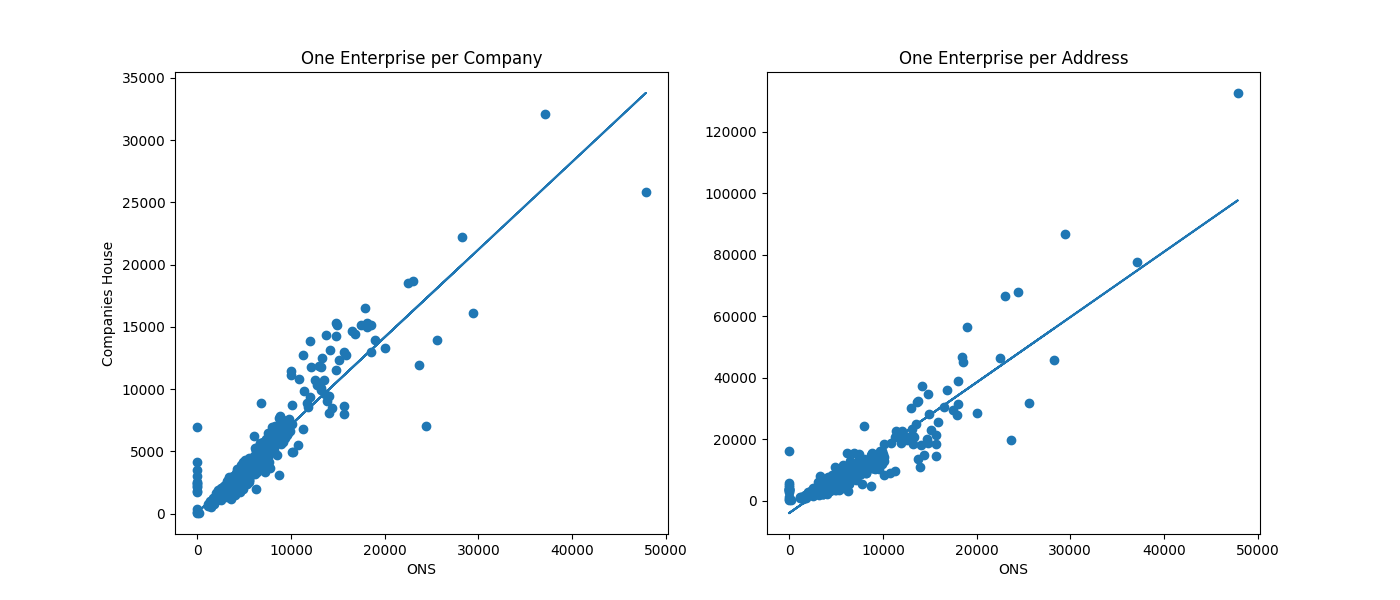
\includegraphics[width=\textwidth]{graphics/filtered_addresses}
 \caption{Improvements in grouping enterprises by addresses}
\end{figure}

After assigning companies to enterprises in this way there is a large number of enterprises missing. This could be because some companies have exempted themselves from reporting to companies house, or an issue with grouping the companies by address. In total for 2017, after the companies have been grouped together there are about 1.6 times as many enterprises as company groups. An effective way to get around this is to assign ratios by SIC code and assume that the enterprises that aren't registered are a representative sample of all the enterprises. We then make the further assumption that this grouping of companies in each SIC code is a representative sample, that is, the distribution of ages and locations by SIC code of the enterprises is the same as the companies groupings. In applying these ratios, the companies house data makes a good prediction for the number of companies in each local authority (figure \ref{predicting number of enterprises}).
\begin{figure}[!ht]
 \begin{center}
 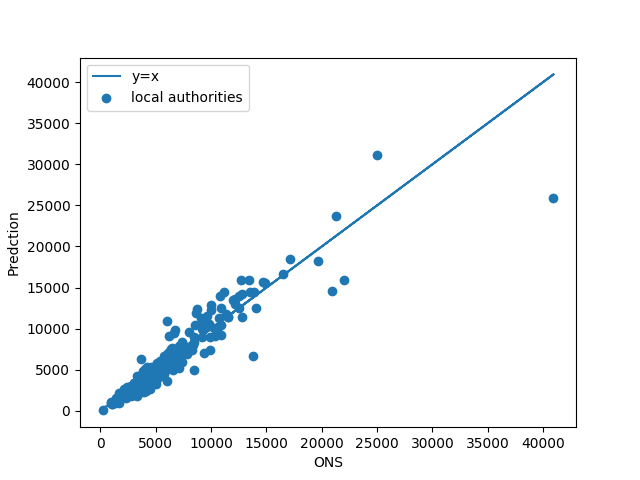
\includegraphics[width=300px]{graphics/la_enterprise_predictions_with_ch}
 \end{center}
 \caption{Predicting the number of enterprises using SIC ratios}
 \label{predicting number of enterprises}
\end{figure}


\subsection{Enterprises Size Distributions}
\label{enterprise_sizes}
ONS release banded employment size data by SIC and local authority individually. Using this data it is possible to fit a log normal distribution\footnote{See appendix, section \ref{ONS size dist parameter fitting}}. To evaluate the log normal hypothesis we compare the expected proportion for each ONS size interval. Generally the fitted distributions work reasonably well for the local authorities, but over estimate the size of the tail of the distribution for SIC codes. As such, when assigning sizes we only use the size bands for each SIC code but generate the actual sizes using the size distributions for each local authority.
\begin{figure}[!ht]
 \caption{Expected proportions for each size band}
\end{figure}

\subsection{Missing Accounts}

\subsection{Predicting turnover}

\section{Assigning Employees}
In order estimate the employment size of each company, we assume that if two companies, $a$ and $b$, have the same SIC code and the turnover of $a < $ the turnover of $b$ then the number of employees of a $a \leq$ the number of employees of $b$. To assign sizes to companies we then perform the following algorithm:
\begin{enumerate}
 \item Using the log normal enterprise size distributions by local authority (\ref{enterprise_sizes}), generate a list of company sizes for each local authority.
 \item For each SIC code, construct a list of the companies house enterprises, ordered by predicted turnover.
\end{enumerate}


\section{Results}
\subsection{Dataset}
\subsection{Total Employment}
\subsection{Employment Migration}

\section{Appendix}
\subsection{Size Bands and Log Normal parameter fitting}
\label{ONS size dist parameter fitting}
The ONS typically release enterprise and local unit size data in bands, so they give the number of companies, $n_i$ with size $x \in [a_i, a_{i+1})$ by some other parameter (SIC code or location). Assuming a log normal distribution where the size X of a company is such that $\log X \sim \mathcal{N}(\mu, \sigma^2)$, $\mu$ and $\sigma$ can be calculated by maximising the log likelihood, given by
\begin{equation}
 l(\mu, \sigma) = \sum_i n_i \log \left( \Phi \left( \frac{\log a_{i + 1} - \mu}{\sigma} \right) - \Phi \left( \frac{\log a_{i} - \mu}{\sigma} \right) \right)
\end{equation}
since $\mathbb{P}(a_i < X < a_{i + 1}) = \mathbb{P}(\log a_i < \log X < \log a_{i + 1}) = \Phi \left( \frac{\log a_{i + 1} - \mu}{\sigma} \right) - \Phi \left( \frac{\log a_{i} - \mu}{\sigma} \right)$. \\
For the employment size distributions of enterprises and local units the the fitted parameters predict the ratios $\frac{n_i}{N}$ well and in the case of local authorities the distributions predict the total employment well so it is perhaps reasonable to assume that the actual distribution is log normal. Whether it is possible for other distributions (Yule or other fat tailed distributions) to reproduce these results is something worth testing, but for the purposes of predicting enterprise and local unit sizes, the log normal distribution seems to work well.




\end{document}
